\chapter{Methodology}

This chapter will indicate the materials, methods and procedures used in the development of the study.
The results and gathered data will be contributed in the development of the automated proctoring application – Proctor Vue.

\section{Methods of Reasearch Used}

The proponents have used the appropriate method in obtaining the data needed in the implementation of the study.
The following are the research methods used in the proposed study.

\section{Descriptive Research Method}

The descriptive method is used to collect facts and information accurately and systematically to describe the people who are taking part to the study.
The researchers used this method to appropriately analyze and interpret relevant information to achieve the aim of the study.

\textbf{Survey Method.}
The proponents used survey method to collect a volume of facts and information that exhibits patterns, relationships and describe something that exist.

\section{Sampling Technique}

The proponents used the probability sampling to utilize the desired form of population selection in the given circumstances.
Probability sampling allows the proponents to create a group of people that is accurately representative of the population of interest of the proposed study.

\textbf{Purposive Sampling.}
this technique is used when a researcher chooses specific and eligible people, fitted in a particular profile within the population to participate in the study.
The relevance of purposive sampling is to leverage individuals that can be identified during the circumstances and to further focus on them in getting the desired data for the effectiveness of the survey method.

\section{Respondents of the Study}

The target respondents of the proposed study are 20 currently enrolled 3rd year IT students taking the full online learning platform of AMA Computer College Parañaque.

\section{Data Gathering instruments}

Data gathering is used by the proponents to gather data from the respondents to further evaluate the proposed study.

\textbf{Surveys.}
The proponents have done online surveys to the selected students to obtain information about their feedbacks and experiences on the current online examination system.

\textbf{Evaluation Form.}
The proponents distributed the evaluation forms to the same set of respondents after they have tested the proposed system.
The proponents used this to gather students’ feedback, evaluation and estimation for the proposed system by means of different criteria and various interpretation.
The data and information gathered will be useful for the adjustments of the proposed system.

\section{Preparation of the Instruments}

The proponents have done efforts to make the gathering of data possible despite the drawback of COVID-19 Pandemic.
Several literatures and studies have been studied to expand their knowledge about the study and to provide the appropriate instruments to be performed to achieve the aim of the study.

\section{Criteria of Software Development}

The following are the software quality characteristics to be used in the software evaluation:

\textbf{Functionality.}
Set of attributes pertaining to the ability of the system’s features to working according to its use.

\textbf{Effectiveness.}
The indication of whether the system is effective in the aim of preventing online cheating during online examination.

\textbf{User Experience.}
The experience of the student users in relation to the smoothness of the program.

\section{Statistical Treatment of Data}

The following tools were used by the proponents to analyze the data gathered on the stated problem.

\begin{table}[h!]
   \begin{center}
      \begin{tabular}{|c|c|c|}
         \hline
         \textbf{Interpretation} & \textbf{Weight} & \textbf{Interval} \\
         \hline
         Strongly Agree          & 5               & 4.21-5.00         \\
         \hline
         Agree                   & 4               & 3.41-4.20         \\
         \hline
         Neutral                 & 3               & 2.61-3.40         \\
         \hline
         Disagree                & 2               & 1.81-2.60         \\
         \hline
         Strongly Disagree       & 1               & 0-1.80            \\
         \hline
      \end{tabular}
   \end{center}
   \caption{5-point Likert’s Scale by Rensis Likert}
\end{table}

\textbf{Likert Scale.}
It measures the statement of agreement of the person by means of a questionnaire that requires them to indicate the extent to which they agree or disagree with a series of statements.

\textbf{Weighted Mean.}
The proponents used the mean to measure the ratings of the respondents regarding on the performance and effectiveness of the proposed system.

\begin{equation*}
   \begin{split}
      \text{Weighted Mean (WM)} & = \frac{\sum f(x1 + x2 + ... + xn)}{N} \\
   \end{split}
\end{equation*}

Where:

\begin{equation*}
   \begin{split}
      \frac{\sum f(x1 + x2 + ... + xn)}{N} & = \text{summation of all means of each criterion} \\
      N & = \text{number of criteria}
   \end{split}
\end{equation*}

\textbf{Percentage.}
This is used to determine the qualitative ratio of the data gathered, it is a number or ratio expressed as a fraction of 100.

\begin{equation*}
   \begin{split}
      \text{Percentage (P)} & = \frac{F}{N} \times 100
   \end{split}
\end{equation*}

Where:

\begin{equation*}
   \begin{split}
      F & = \text{frequency of a numeric rating for some given criteria} \\
      N & = \text{represents the total number of the respondents}
   \end{split}
\end{equation*}

\section{Analytical Tools}

This section discusses the tools used to design, analyzed, and develop the proposed Web-based automated proctor.
The following are the instruments with their descriptions.

\textbf{Program Flowchart.}
A diagram which uses set of standard symbols to represent the sequence of operations of the software.
This provided the proponents to view the proposed system in a sequenced operation manner using the set of standard symbols.

\begin{figure}[h!]
   \begin{center}
      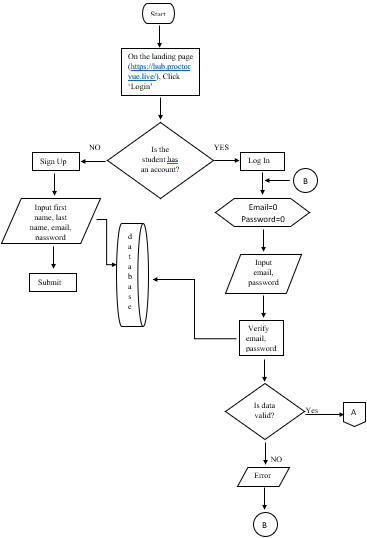
\includegraphics[scale=1.3]{fc1}
      \caption{Program Flowchart}
   \end{center}
\end{figure}

\pagebreak

\begin{figure}[h!]
   \begin{center}
      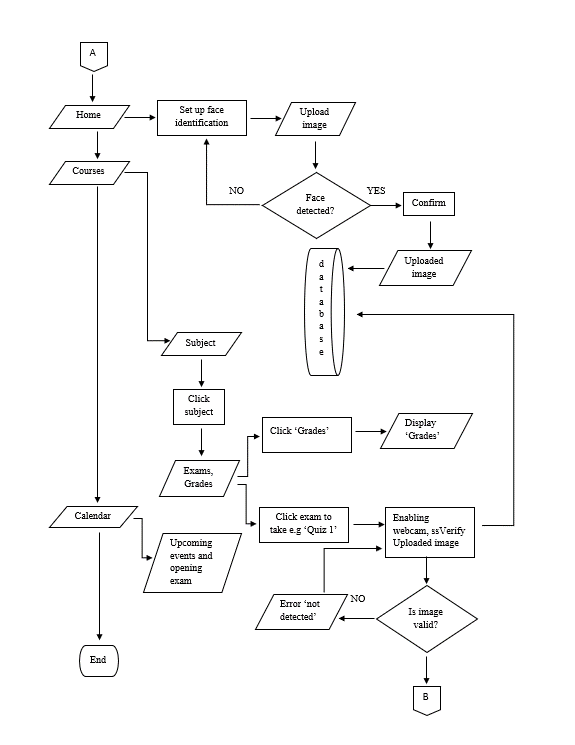
\includegraphics[scale=1.3]{fc2}
      \caption{Program Flowchart}
   \end{center}
\end{figure}

\pagebreak

\begin{figure}[h!]
   \begin{center}
      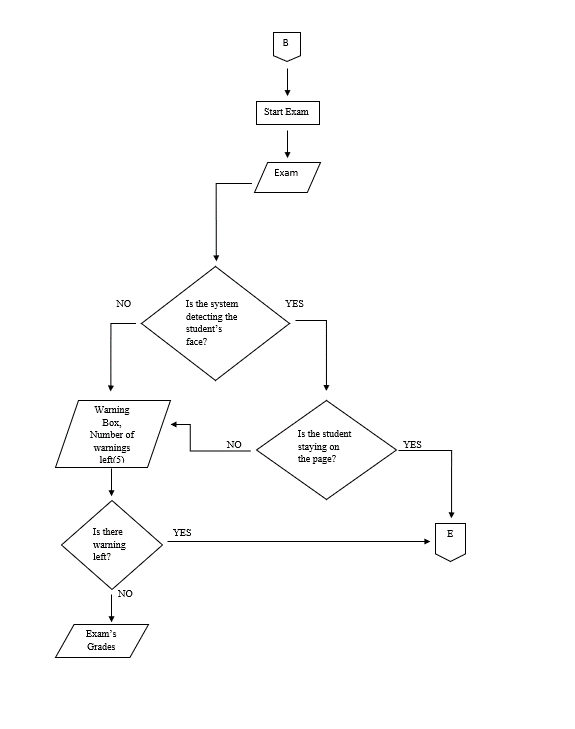
\includegraphics[scale=1.4]{fc3}
      \caption{Program Flowchart}
   \end{center}
\end{figure}

\pagebreak

\begin{figure}[h!]
   \begin{center}
      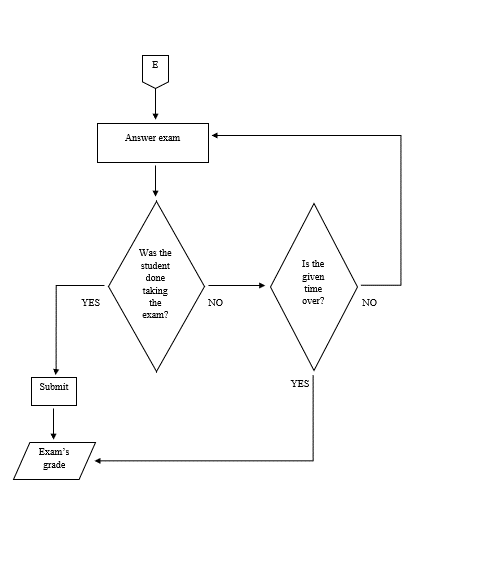
\includegraphics[scale=1.4]{fc4}
      \caption{Program Flowchart}
   \end{center}
\end{figure}

% \textbf{Storyboard.}
% It is a graphic organizer that provides the viewer with a high-level view of a project.
% This helped the proponents to visualize the proposed system through a story-type of illustration

\section{Software Model}

This section will discuss the process of evaluating the problem and building a solution as the proposed study.

\pagebreak

\begin{figure}[h!]
   \begin{center}
      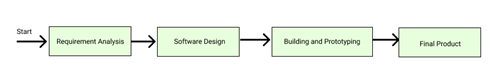
\includegraphics[scale=0.9]{prototyping-model}
      \caption{Prototyping Model}
   \end{center}
\end{figure}

The following are the methods and procedures used by the proponents in the implementation of the proposed system.

\textbf{Phase 1. Requirement Analysis.}
Requirement Analysis, also known as Requirement Engineering, is the process of defining user expectations for a new software being built or modified.
In software engineering, it is sometimes referred to as requirements gathering or requirements capturing such that determining the needs or conditions to meet for a new or altered product or project.
The proponents based the requirements needed on the current system of online examination of AMA Computer College Parañaque.

The following Data-Flow Diagram (DFD) illustrates the requirements needed to build and develop the proposed system.

\pagebreak

\begin{figure}[h!]
   \begin{center}
      \includegraphics[scale=0.5]{dfd.jpg}
      \caption{Data Flow Diagram of the Proposed System}
   \end{center}
\end{figure}

\textbf{Phase 2. Software Design.}
After determining the requirements needed, a system design is created.
This includes the important aspects of the system to the user.
The proponents aim to design the Proctor Vue: Automated online proctor Web application with four(4) major sections: (1) Authentication, (2) Settings, (3) Home, (4) Courses.

The software design of the proposed system is represented by the following Hierarchical Input-Process-Output (HIPO) diagrams

\pagebreak

\begin{figure}[h!]
   \begin{center}
      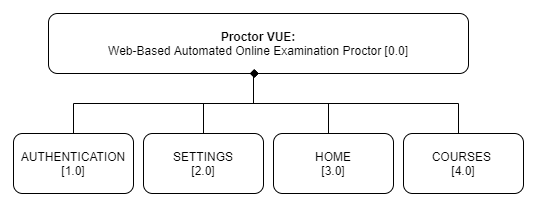
\includegraphics[scale=0.8]{main-hipo}
      \caption{Proctor Vue HIPO}
   \end{center}
\end{figure}

\vspace{1cm}

\begin{figure}[h!]
   \begin{center}
      \includegraphics[scale=0.7]{auth-hipo.png}
      \caption{Authentication}
   \end{center}
\end{figure}

\vspace{1cm}

\begin{figure}[h!]
   \begin{center}
      \includegraphics[scale=0.7]{home-hipo.png}
      \caption{Home Page}
   \end{center}
\end{figure}

\vspace{1cm}

\begin{figure}[h!]
   \begin{center}
      \includegraphics[scale=0.7]{courses-hipo.png}
      \caption{Courses}
   \end{center}
\end{figure}

\vspace{1cm}

\begin{figure}[h!]
   \begin{center}
      \includegraphics[scale=0.7]{settings-hipo.png}
      \caption{Settings}
   \end{center}
\end{figure}

\textbf{Phase 3. Prototyping.}
The created system design derived from the requirements is modified to for the system’s prototype.

Proctor Vue will implement facial detection/recognition during online exams for different courses.
These exams will be created by the assigned coordinator in each course through Proctor Vue.
Before users can take the exams, they must provide an image of themselves in order for the camera to ensure they are the ones present for their examination.
During an exam, the student’s face must be seen and recognized as the provided image every minute or else they will incur a warning.
Maxing out the set number of warnings for the exam will automatically fail the student for that attempt.

\textbf{Phase 4. Final Product.}
Given the methods and procedures used, the proposed software is considered final and is available for use.
After performing a number of tests, the software is deployed.
The final product is then evaluated by the selected students by means of effectiveness, functionality and user experience.

\section{System Features}

In this section, the features of the Proctor Vue: Web-based Automated Online Proctor will be discussed.

\textbf{Face recognition}

Through Artificial Intelligence, the proposed system can verify if the person taking the exam is the registered face of the student in the account.

\textbf{Alt-tab switching detection}

The proposed system will recognize if the examinee is trying to switch their tabs through patterns of behavior made by the student.

\section{Cost Benefit Analysis}

% \noindent
% \textbf{Software Development Cost}

% \begin{table}[h!]
%     \begin{center}
%         \begin{tabular}{|l|c|r|}
%             \hline
%             \textbf{Personnel}                   & \textbf{No. of Personnel} & \textbf{Salary} \\
%             \hline
%             Programmer                           & 1                         & \PHP20,000.00   \\
%             \hline
%             System Analyst                       & 1                         & \PHP35,000.00   \\
%             \hline
%             \multicolumn{2}{|l|}{\textbf{Total}} & \textbf{\PHP55,000.00}                      \\
%             \hline
%         \end{tabular}
%     \end{center}
%     \caption{Software Development Cost}
% \end{table}

% \noindent
% \textbf{System Cost}

\begin{table}[h!]
   \begin{center}
      \begin{tabular}{|l|c|r|}
         \hline
         \textbf{Item}                        & \textbf{Specification}       & \textbf{Cost} \\
         \hline
         Datebase Instance                    & MongoDB Atlas                & \PHP2,805.81  \\
         \hline
         Storage for User-Uploaded Images     & Amazon S3/CloudFront         & \PHP32.15     \\
         \hline
         Web Application Hosting              & Amazon S3/CloudFront         & \PHP454.82    \\
         \hline
         Load Balancer                        & Amazon Elastic Load Balancer & \PHP896.30    \\
         \hline
         Application Backend and API          & Amazon EC2                   & \PHP4,246.70  \\
         \hline
         \multicolumn{2}{|l|}{\textbf{Total}} & \textbf{\PHP8,435.78}                        \\
         \hline
      \end{tabular}
   \end{center}
   \caption{System Cost}
\end{table}

Source: www.mongodb.com, calculator.aws

\section{Description of the Prototype}

Proctor Vue will implement facial detection/recognition during online exams for different courses.
These exams will be created by the assigned coordinator in each course through Proctor Vue.
Before users can take the exams, they must provide an image of themselves in order for the camera to ensure they are the ones present for their examination.
During an exam, the student's face must be seen and recognized as the provided image every minute or else they will incur a warning.
Maxing out the set number of warnings for the exam will automatically fail the student for that attempt.

\section{Implementation Plan}

The developed system will be sent to AMA Computer College Parañaque right away after the revision to present it once more to the end users.
If the company wants to adopt the proposed system, the proponents will hand over the system together with its documentation which will serve as a guide to the Administrator who will be assigned for the system’s update and maintenance.
There will be a letter of agreement that the system will be handed over to the company freely and the researchers are no longer responsible for the updates and maintenance.

If the system will be implemented, the researchers will conduct several strategies as presented below

\vspace{1cm}

\begin{table}[h!]
   \begin{center}
      \begin{tabular}{|m{10em}|m{8em}|m{10em}|m{4em}|}
         \hline
         \textbf{Strategy}        & \textbf{Activities}              & \textbf{Persons Involved}         & \textbf{Duration} \\
         \hline
         Approval from Admin      & Send letter to Admin             & Researchers \& Admin              & 1 Day             \\
         \hline
         Information distribution & Provide techinical documentation & Researchers \& Admin              & 1 Day             \\
         \hline
         3 Days training          & Training for users               & Researchers \& Admin \& Employees & 3 Days            \\
         \hline
      \end{tabular}
   \end{center}
   \caption{Implementation Plan}
\end{table}
